\begin{figure}[htbp]
    \caption{Impact of Contributor Departures by Other Collaboration}
    \label{fig:prs_opened_other_fig}
    \centering
    \begin{minipage}[b]{0.48\textwidth}
        \centering
        \subcaption{By other collaboration} \label{fig:prs_opened_other}
        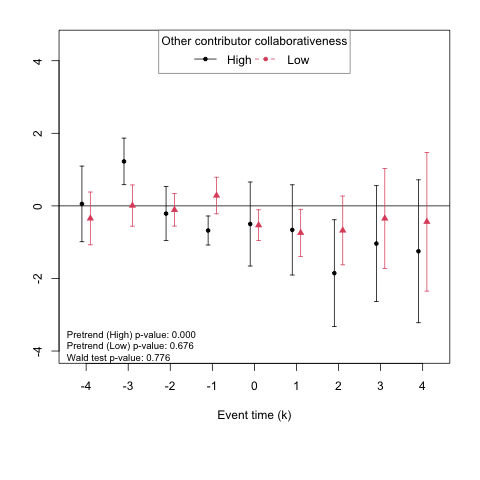
\includegraphics[width=\textwidth]{temp/output/collab/prs_opened_other_collab_cs_norm.png}
    \end{minipage}
  \begin{minipage}{\textwidth}
    \textbf{Figure notes:} 
    Following Callaway and Sant’Anna (2021), I estimate event-study coefficients accompanied by 95\% simultaneous confidence bands. For each plot with event study estimates from two subsamples, I report three Wald-test p-values: one for the pretrend test in the first subsample, one for the pretrend test in the second subsample (both from Equation \ref{eq:wald_test_pretrends} in Section \ref{sec:main_method}), and one for the difference in treatment effects across subsamples (Equation \ref{eq:wald_test} in Section \ref{sec:att_subset}). 
    Panel~\subref{fig:prs_opened_other} plots two sets of event study estimates: projects with high and low collaboration among other key contributors (as defined in Section~\ref{sec:collab_imp_contr}). In all panels, the outcome is the pull request z score, transformed using the pre-treatment mean and standard deviation.

  \end{minipage}
\end{figure}
